\documentclass[conference]{IEEEtran}
\usepackage[utf8]{inputenc}
\usepackage{graphicx}
\usepackage{svg}


% correct bad hyphenation here
\usepackage{cite}
\hyphenation{op-tical net-works semi-conduc-tor}

\DeclareUnicodeCharacter{00A0}{~}

\begin{document}
%
% paper title
% can use linebreaks \\ within to get better formatting as desired
\title{Traffic Lane Detection in Urban Environments}


\author{\IEEEauthorblockN{Marin Vlastelica Pogančić}
\IEEEauthorblockA{Karlsruher Institüt für Technologie\\
Karlsruhe, Deutschland\\
Supervisor: Florian Kuhnt}}


% make the title area
\maketitle


\begin{abstract}
%\boldmath
We live in a time of rapid development of autonomous driving systems and the continuous deployment of the same systems in everyday life. This poses a large span of challenges, in order to make the systems reliable and robust in their deployment, much of this robustness relies on the information obtained through sensors from the environment. The pros and cons of different approaches for traffic lane detection will be discussed and the corresponding results compared, with an emphasis on the urban environment, where the challenge of detecting the lanes requires more consideration. 
\end{abstract}



\IEEEpeerreviewmaketitle



\section{Introduction}

As mentioned in the abstract, lane traffic detection in urban environments poses an even greater challenge, there are many reasons for this. One of the main reasons is the cluttered environment, urban environments have many objects, obstacles on the streets which can contribute to the ambiguity of the sensor data. On the other hand, we have many streets in urban environments that don't have lane markings, which means that robust curb detection is also needed to detect the traffic lanes correctly. In chapter II are the lane marking methods discussed. In chapter III are the curb detection methods discussed. 

\subsection{Diverse Approaches}

Diverse solutions for the lane detection problems exist since a long time ago, most of them based on 3D data analysis and pattern recognition. The challenge is to improve the robustness of the detection algorithms using additional context. Therefore, there are some approaches using vehicle tracking to determine the positions of the markings, like proposed in \cite{virtuallane}, that try to use additional context to make the detections more robust and effective. Albeit there are many approaches in this field, the sensor data in use is not so diverse, the driving lane detection is mostly based on stereo-camera imagery and 3D laser sensor data.


\section{Lane Marker Detection}

\subsection{Lane Detection Enhancement Using Virtual Lane}

In this section will a method be described, that uses relative movements between the vehicles to enhance the lane detection. This approach is meant to overcome the difficulties that pose themselves through pure detection through the camera. In comparison to the other  



\section{Road Curb Detection}

One of the more important tasks in an urban environment is curb detection. The reason for this is that many streets in an urban environment are small streets without lane markings. In order to fully function in an urban environment, autonomous vehicles have to solve this problem in an appropriate manner also. In this chapter will the different approaches to solving this problem be mentioned.  

\subsection{Elevation Mapping Techniques With Stereo Camera}

In this chapter will an approach suggested in \cite{stereo} be explained. The approach, as the name suggests, is based on using elevation maps. By means of these maps can the most probable paths be calculated. The position accuracy that was able to be achieved is about 10 cm and an height error of about 1.5 cm, tested in real-time.

The sensor used primarily in this approach is the stereo camera, where the output of the stereo camera are two intensity images and one disparity image. For the ego motion is the inertial measurement unit used. 

The first step that is to be made is to take the disparity image and generate a position 3D point cloud from it in the sensor coordinate system. This generated point cloud finds itself in the sensor coordinate system at the beginning, the next step is to transform this point cloud into the map coordinate system after the ground pixels had been detected. Thereafter is important to use the ego motion estimation. 

The ego motion estimation is used to estimate the ego motion of the vehicle between two timestamps. The DEM model used in this approach is based on a 2.5-D map described in \cite{bewegung}. It accumulates of the stereo camera in the Euclidean space using temporal integration. One cell in the map is of the size 20 x 20 cm and has a one dimensional Kalman-Filter which estimates the height of the cell. In each prediction step is the cell height adjusted according to the ego motion of the car, for the correction step is the Kalman-Filter updated with the sensor measurements. 

The detection approach is as follows. The static and dynamic objects lead to value spikes in the DEM, whereby the dynamic objects need to be removed, in order to detect the curbs. The dynamic objects are detected with a laser scanner and removed from the point cloud generated from the stereo camera.The rest of the points are divided into ground points and object points. The ground detection algorithm assumes steadily growing x values in the sensor coordinate system, when the disparity image columns are considered. If the x values are steadily growing, then it can be assumed, that ground is in front of the car, otherwise this assumption cannot be made. To compensate the effect of the outliers, the mean value of two consecutive columns with 3 pixels each is calculated.

What also must be considered are the mapping techniques which also have an effect on the performance, since these are not the central aspect of this paper, all of them are mentioned and analysed in \cite{stereo}. 

The road curb is represented by a polygonal chain, this chain consists of supporting points and the connections between these supporting points. Every point contains a 2D position and the road curb height at its position. 

\subsubsection{Road Curb Detection Algorithm}

The first step at road curb detection is the road curb feature extraction. This is achieved by applying an edge-detection algorithm on the DEM to find cells with a jump in the neighbouring height values, which might be caused by a road curb. Only cells with a minimal number of updates are considered, because less updates means more noise. A Sobel operator is used for the edge detection an the result is normalized, if the normalized result finds itself within a range, then a road curb feature is found.

In the next step the features are registered in a second map with the size of the region of interest and a lower resolution.There must be a minimum of features in one of the low resolutions cells to be marked as a curb cell, because a road curb is not a singular feature like a reflector post used for road boundary detection. By building histograms of road curb features perpendicular to the driving direction the most probable path is determined. To build the polygonal chain the minimal distance approach is used,which considers the closest features to the most probable path as the road curb. In general the road curb is the closest boundary to the path visible in an elevation map. The output of the road curb detection algorithm are polygonal chains for both sides of the vehicle.


\subsection{Laserscanner Based Road Curb Detection}

In this section a method proposed in \cite{stereo} using a laser scanner to detect road curbs will be described. The argument for using laser scanners instead of stereo cameras is that the laserscanner provides more accurate data. Some methods have been developed, that use sensor fusion with the stereo camera to overcome this precision lacking. Unfortunately these methods produce a big overhead in the data processing step, which makes a big difference in an autonomous vehicle, because it is a real-time system.

For testing this method, the equipment proposed in \cite{stereo} is the following. For road curb detection, a multipurpose laserscanner is used. For the ego motion estimation a low cost inertial measurement unit is used in combination with the standard wheel speed sensors and chassis lift sensors. 

The road curb detection pipeline is shown in \ref{fig1}. As the figure shows, the detection is split into 3 modules. In the first module is used for for the road curb feature extraction and labeling. The detected road curb candidates have to be accumulated over time, so they are stored into the road curb map, where they undergo ego motion compensation. In the last module uses the temporal filtered parameters stored in the cells of the road curb map to group the road curb candidates into road curbs. In the end, the road curbs are represented as polygonal chains.  

\begin{figure}[ht]
	\centering
  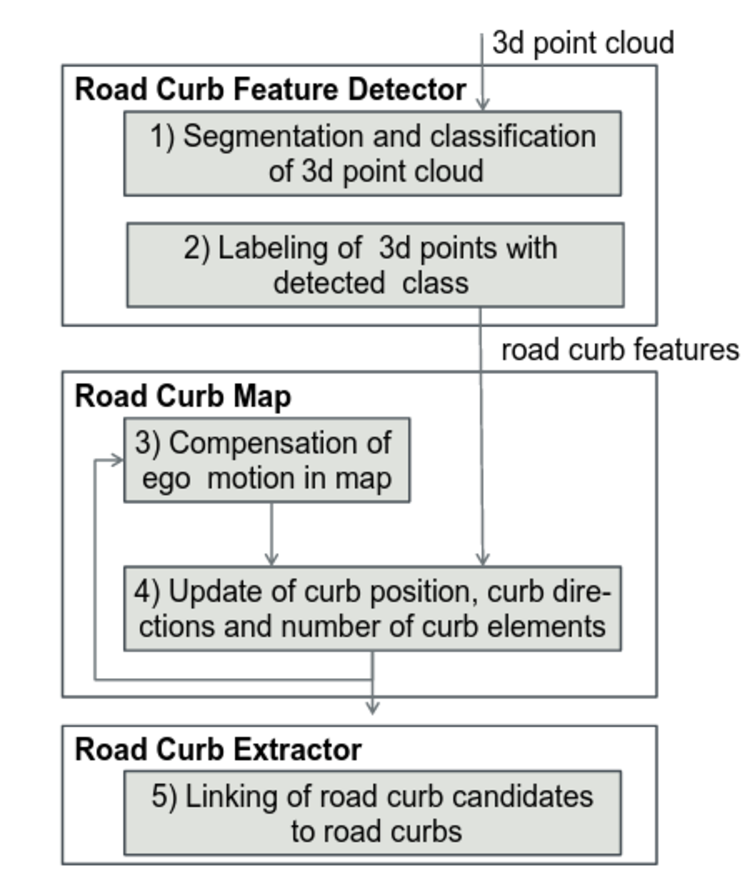
\includegraphics[scale = 0.5]{pictures/lidar_system.pdf}
	\caption{Ro}
	\label{fig1}
\end{figure}
  
At the point of detecting road curb features, three approaches can be used: segmentation using iterative end point fit and classification of segments, hierarchic segmentation and classification of segments, segmentation using regression lines and classification of segments.

The IEPF algorithm described in this section is a well known segmentation algorithm. In this method, the input to the algorithm is the orthogonal projections of the 3D points on the y-z plane. The start and end point of the scan line are connected and the distance to the straight line is calculated for each point, as shown in \ref{fig2}. The measurement points are split into two segments at the point with maximum distance, the circled point in \ref{fig2}, if it exceeds a predetermined threshold. This takes place for every generative segment iteratively, till there are no points that cross this threshold. For each segment that contains the minimum number of points, the angle $\alpha_S$ between the regression line of the segments, the average height and the variance of the height values is being calculated. The segments are classified into four classes: road curb, object, ground and street. This method assumes that the segments containing the central channels of the scan lines is a street. After that, the process continues by going in both direction of the scan line and classifying the object segment with a object classification algorithm. For the segments not labeled as objects, an angle between that segment and the last found street segment is calculated. If this angle $|\alha - \alpha_S|$ is greater than a threshold $T_{\alpha,1}$, the segment is marked as a road curb. If the angle is greater than $T_{\alpha,2}$ but lower than $T_{\alpha,1}$, or the difference to the height of the neighboring lane segment $|h - h_S|$ is lower than $T_h$ or the difference in variance $|\sigma - \sigma_S|$ is above $T_\sigma$, then the segment is marked as ground. The variance criterion is used to distinguish the streets in unstructured environments, with a lot of gravel and grass for example. If none of these criteria are met, then the segment is classified as a street segment and is used for further evaluation of segments. 

\begin{figure}[ht]
	\centering
  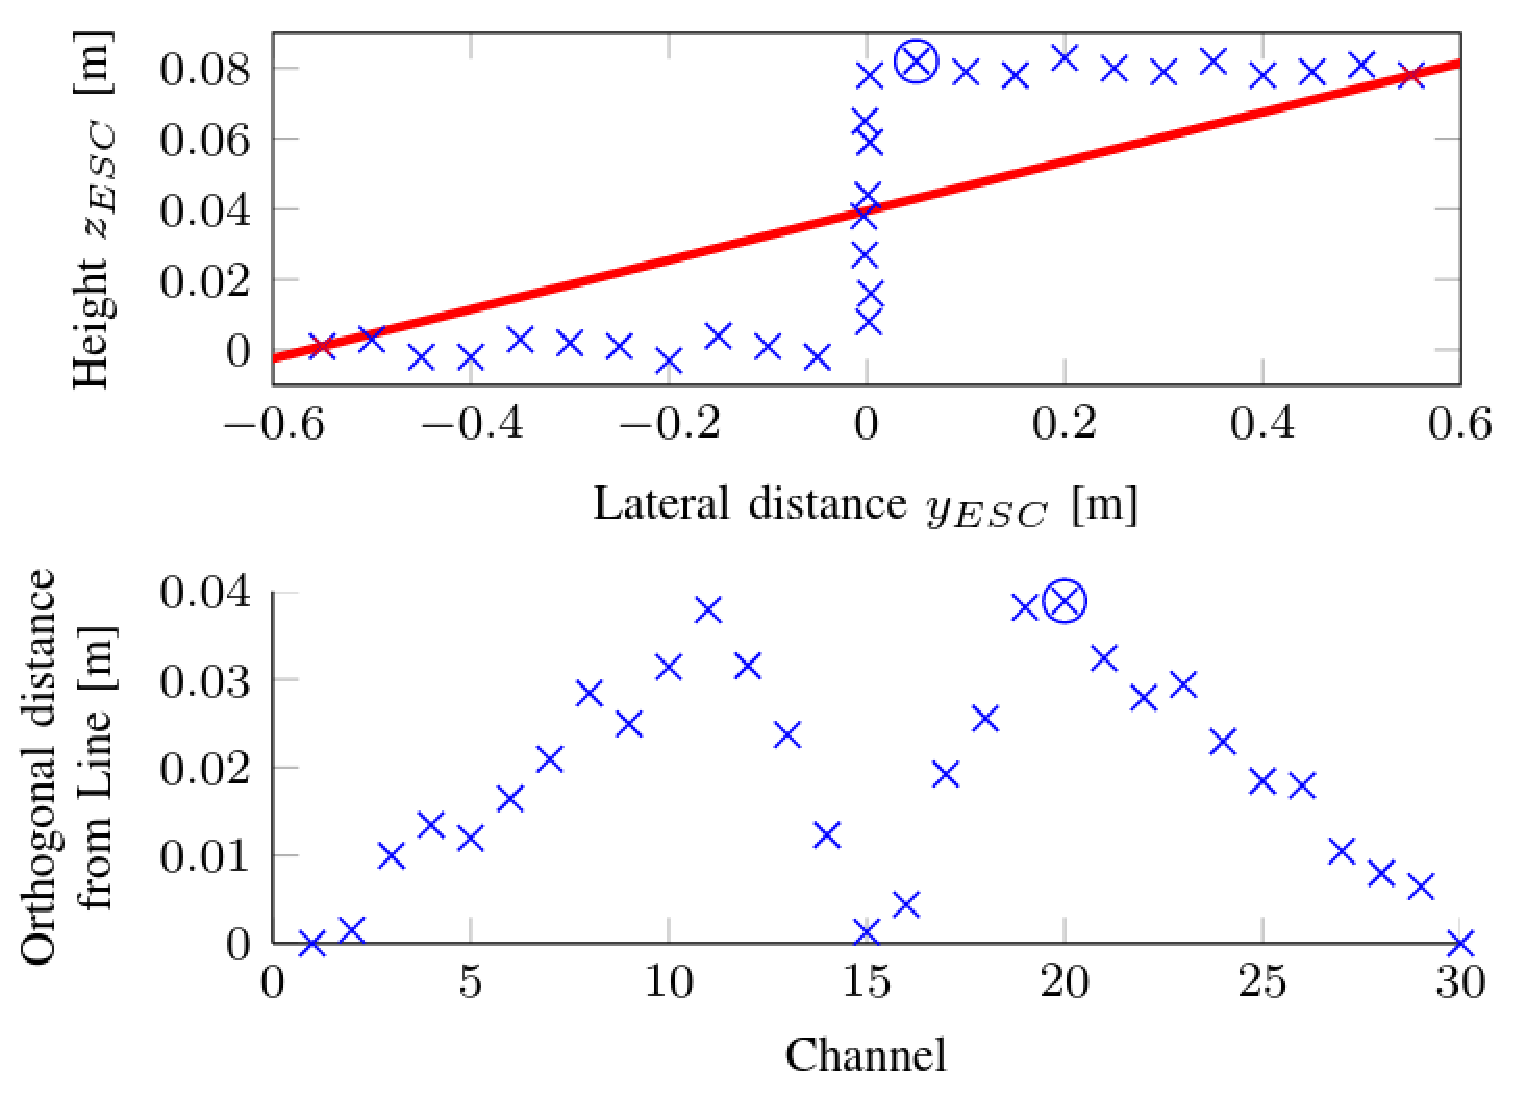
\includegraphics[scale = 0.35]{pictures/iepf.pdf}
	\caption{Ro}
	\label{fig2}
\end{figure}
 

Another possible approach for segmentation is segmentation using regression lines. For every measurement point a forward anda backward regression line is calculated containing n pointsbefore or after the measurement point. The regression lines are calculated in the z-channel-space.  In all adjunct points with anintersection angle exceeding a certain threshold a maximum search regarding the intersection angle is conducted. At the maximum, a segment is terminated. The classification steps are performed in the y-z-space again as described for the IEPF algorithm. As the regressions lines are build with only a few measure-ment points this detection algorithm is sensitive to outliers inthe data set? This segmentation method is shown in \ref{fig3}

\begin{figure}[ht]
	\centering
  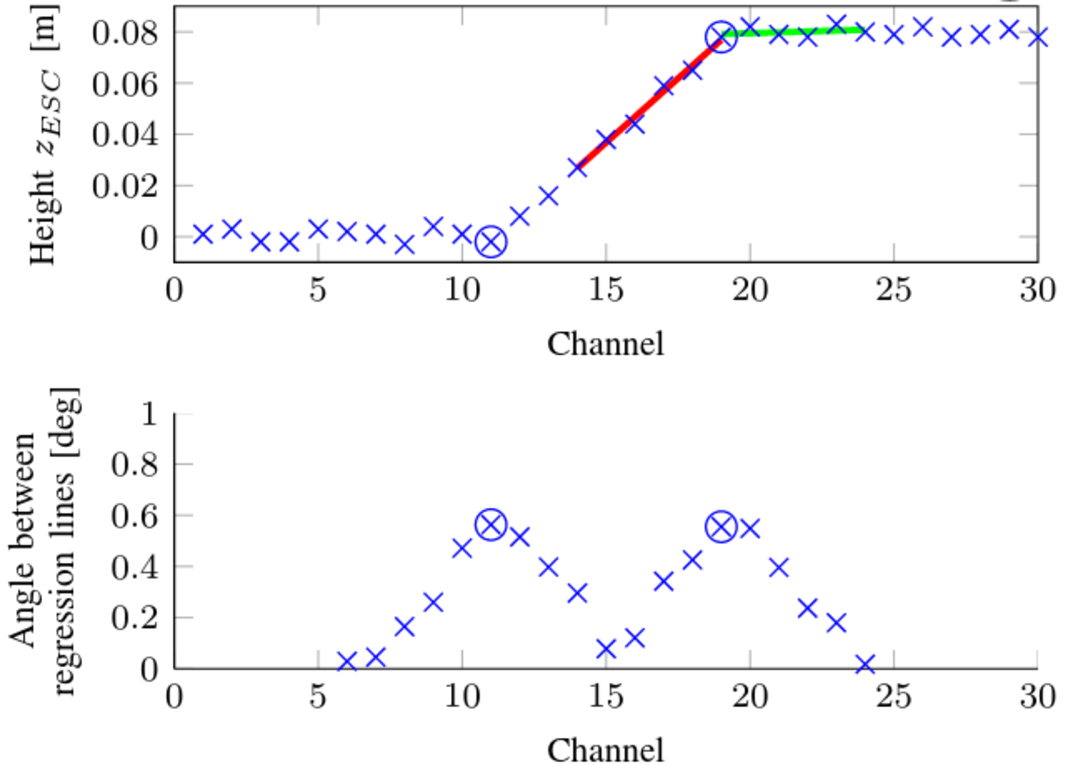
\includegraphics[scale = 0.5]{pictures/iepf2.pdf}
	\caption{Ro}
	\label{fig3}
\end{figure}

The final segmentation method considered is the hieararchic segmentation and classification of segments. The segments are built pairwise from neighboring height values. Two neighboring segments are merged if the standard deviation of the height values in relation to the calculated regression line of the merged segment is below a certain threshold. This is processed in a pyramid procedure until a new segment does not fulfill the described variance criterion.This process ist shown in \ref{fig4}

\begin{figure}[ht]
	\centering
  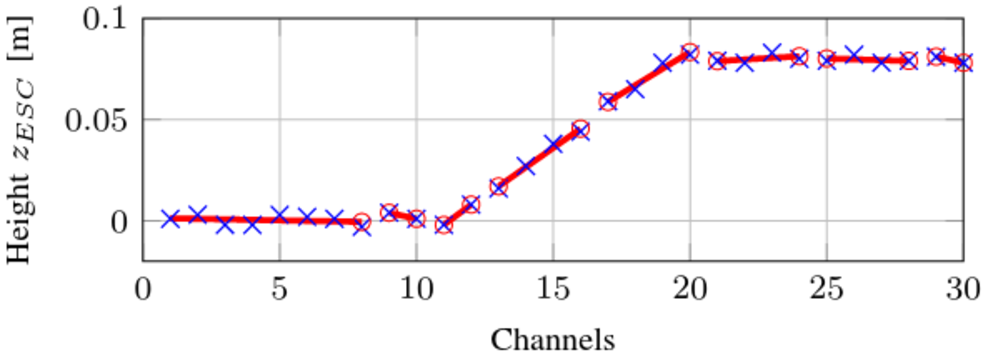
\includegraphics[scale = 0.55]{pictures/iepf3.pdf}
	\caption{Ro}
	\label{fig4}
\end{figure}

The cells of the grid based road curb map contain a local description o the road curb based on a linear model. Each cell contains the model parameters center point $(x^C, y^C)$ and direction $d = (1, \beta_1)^T$, and additionally the number of cell updates n.The model parameters are updated with every curb feature lying in the cell. Of course this is not enough to achieve a precise road curb estimation so the centers of the road curbs are estimated within the cell.

The larger the cell is, the better the computation time and memory consumption. Large cells are good for straight road curbs, but smaller cells are better for road curbs with complex geometry.

For every new measurement frame an additional step is necessary to compensate the ego motion between two measurement time stamps(reference). 

The road curb extraction takes place in the road curb extraction module. The module uses the model parameters to build chains of road curb candidates. To identify the most relevant curb chains, an estimated central line of the current lane is used, as shown in \ref{fig5}

\begin{figure}[ht]
	\centering
  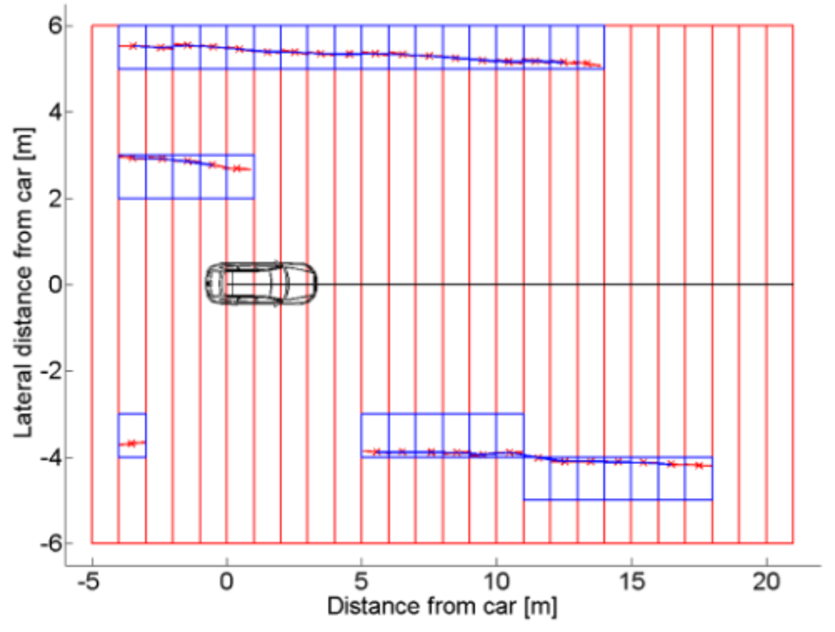
\includegraphics[scale = 0.6]{pictures/extractor.pdf}
	\caption{Ro}
	\label{fig5}
\end{figure}

\section{Conclusion}
The conclusion goes here.
\nocite{*}

% use section* for acknowledgement
\section*{Acknowledgment}

The authors would like to thank...


\bibliographystyle{bibtex/IEEEtran}
\bibliography{bibliography}

% that's all folks
\end{document}


